% Chapter 5 — Experimental Results

\chapter{Experimental Results}
\label{chap:results}

This chapter reports the empirical behavior of the algorithms introduced in
Chapter~3. The presentation is organized around recurring patterns rather than
around the complete set of generated plots. The one-player experiments show
how the three regret notions respond to changes in the reward process, the
action-space size, and the horizon; the repeated-game experiments add self-play,
cross-play, and empirical CE/CCE behavior. Supplementary trajectory views,
individual horizon-scaling fits, selected action-space examples, and selected
repeated-game profiles are collected in
Appendix~\ref{app:supplementary-results}.

Section~\ref{sec:one-player-results} covers the historical-frequency and
lazy-random-walk reward processes together with the action-space and horizon-
scaling studies.
Section~\ref{sec:self-play-results} then considers self-play and cross-play
in RPSLS and RPS. The discussion in this chapter remains descriptive; the
connection to the theoretical results
from earlier chapters is taken up in Chapter~6. Unless stated otherwise, the
comparative statements below refer to the tested environments and game
instances rather than to the corresponding classes in general. The plotted
curves and endpoint comparisons are replicate means; small differences between
nearby endpoints are therefore treated descriptively rather than as evidence
of a statistically established ranking.

\section{One-Player Regret Experiments}
\label{sec:one-player-results}

This section compares the one-player experiments across reward processes,
action-space sizes, and horizons. The main text focuses on representative
comparisons, while supplementary trajectory views, individual horizon-scaling
fits, and selected action-space examples are collected in
Appendix~\ref{app:one-player-results}. Unless stated otherwise, regret
trajectories use $R_T/T$, i.e., average regret per round; supplementary
$R_T/\sqrt{T}$ views in Appendix~\ref{app:one-player-trajectories} are used
where this normalization makes finite-horizon differences easier to distinguish.


% ============================================================
\subsection{Comparison Across Environments}
\label{sec:one-player-overview}

The two reward processes exhibit markedly different degrees of separation
among the tested learners. The historical-frequency environment provides the
higher-contrast case, whereas many of these differences are compressed in the
lazy random walk. We therefore begin with the historical-frequency results
before comparing the corresponding behavior under the lazy-random-walk
environment.

\paragraph{Historical-frequency environment.}

Figure~\ref{fig:hfa-overview} compares external and swap regret under both
feedback models.

\begin{figure}[H]
    \centering

    \begin{subfigure}{0.43\textwidth}
        \centering
        \includegraphics[
            page=2,
            width=\linewidth
        ]{figures/regret/hfa/algorithm_comparison_full_information.pdf}
        \caption{Full information, external regret}
    \end{subfigure}
    \hfill
    \begin{subfigure}{0.43\textwidth}
        \centering
        \includegraphics[
            page=2,
            width=\linewidth
        ]{figures/regret/hfa/algorithm_comparison_bandit.pdf}
        \caption{Bandit, external regret}
    \end{subfigure}

    \begin{subfigure}{0.43\textwidth}
        \centering
        \includegraphics[
            page=10,
            width=\linewidth
        ]{figures/regret/hfa/algorithm_comparison_full_information.pdf}
        \caption{Full information, swap regret}
    \end{subfigure}
    \hfill
    \begin{subfigure}{0.43\textwidth}
        \centering
        \includegraphics[
            page=10,
            width=\linewidth
        ]{figures/regret/hfa/algorithm_comparison_bandit.pdf}
        \caption{Bandit, swap regret}
    \end{subfigure}

    \caption{External and swap regret in the historical-frequency environment.}
    \label{fig:hfa-overview}
\end{figure}

Under full information, most algorithms become tightly concentrated under
the external benchmark. RM is the main exception, while the remaining
learners occupy a comparatively narrow region toward the end of the run.
Under swap regret, the broad separation is already visible in
Figure~\ref{fig:hfa-overview}, although the late-horizon differences are
compressed by the \(R_T/T\) normalization. The supplementary
\(R_T/\sqrt{T}\) view in Figure~\ref{fig:app-oneplayer-swap-sqrt} makes the
grouping clearer: Hedge and OptHedge remain well above BM-Hedge, Ito-Hedge,
SRM, and BM-OptHedge.

The bandit comparison shows the same broad contrast. The external-regret
trajectories remain comparatively close, whereas under swap regret EXP3 and
EXP3-IX form the upper group, BM-EXP3 and Ito-Tsallis occupy an intermediate
range, and LCE-IX lies below them.

Thus, the empirical grouping of the algorithms changes with the regret
notion; the differences visible under swap regret are not reproduced by a
simple rescaling of the external-regret plot.


\paragraph{Lazy-random-walk environment.}

Figure~\ref{fig:lrw-overview} shows the corresponding external- and
swap-regret comparisons for the lazy-random-walk environment. The separation
among the tested learners is considerably smaller than in the
historical-frequency case.

\begin{figure}[H]
    \centering

    \begin{subfigure}{0.43\textwidth}
        \centering
        \includegraphics[
            page=2,
            width=\linewidth
        ]{figures/regret/lrw/algorithm_comparison_full_information.pdf}
        \caption{Full information, external regret}
    \end{subfigure}
    \hfill
    \begin{subfigure}{0.43\textwidth}
        \centering
        \includegraphics[
            page=2,
            width=\linewidth
        ]{figures/regret/lrw/algorithm_comparison_bandit.pdf}
        \caption{Bandit, external regret}
    \end{subfigure}

    \begin{subfigure}{0.43\textwidth}
        \centering
        \includegraphics[
            page=10,
            width=\linewidth
        ]{figures/regret/lrw/algorithm_comparison_full_information.pdf}
        \caption{Full information, swap regret}
    \end{subfigure}
    \hfill
    \begin{subfigure}{0.43\textwidth}
        \centering
        \includegraphics[
            page=10,
            width=\linewidth
        ]{figures/regret/lrw/algorithm_comparison_bandit.pdf}
        \caption{Bandit, swap regret}
    \end{subfigure}

    \caption{External and swap regret in the lazy-random-walk environment.}
    \label{fig:lrw-overview}
\end{figure}

Under full information, the swap-regret curves are much more tightly grouped
than in the historical-frequency environment. This late-horizon ordering is
again clearer under the \(R_T/\sqrt{T}\) normalization in
Figure~\ref{fig:app-oneplayer-swap-sqrt}: Hedge, OptHedge, and BM-Hedge occupy
a similar range, while Ito-Hedge, SRM, and BM-OptHedge remain near the lower
end of the comparison. RM remains visibly above the other methods.

The compression is even more striking under bandit feedback. EXP3,
EXP3-IX, BM-EXP3, Ito-Tsallis, and LCE-IX remain close under external regret
and also finish in a narrow range under swap regret. The three-level grouping
visible in the historical-frequency experiment largely disappears.

The contrast with HFA is not a uniform shift in regret magnitude. Across the
two tested reward processes, both the amount of separation and several
pairwise orderings change.


% ============================================================
\subsection{Relations Among Regret Notions}
\label{sec:regret-notion-relations}

The aggregate plots compare algorithms one regret notion at a time. Viewing
all three notions for the same learner exposes a complementary feature of the
data: internal regret often evolves differently from external and swap regret.
Figure~\ref{fig:regret-notion-shapes} illustrates this for Hedge and EXP3 in
both environments.

\begin{figure}[H]
    \centering

    \begin{subfigure}{0.43\textwidth}
        \centering
        \includegraphics[
            page=10,
            width=\linewidth
        ]{figures/regret/hfa/regret_curves_full_information.pdf}
        \caption{HFA, Hedge}
    \end{subfigure}
    \hfill
    \begin{subfigure}{0.43\textwidth}
        \centering
        \includegraphics[
            page=2,
            width=\linewidth
        ]{figures/regret/hfa/regret_curves_bandit.pdf}
        \caption{HFA, EXP3}
    \end{subfigure}

    \begin{subfigure}{0.43\textwidth}
        \centering
        \includegraphics[
            page=10,
            width=\linewidth
        ]{figures/regret/lrw/regret_curves_full_information.pdf}
        \caption{LRW, Hedge}
    \end{subfigure}
    \hfill
    \begin{subfigure}{0.43\textwidth}
        \centering
        \includegraphics[
            page=2,
            width=\linewidth
        ]{figures/regret/lrw/regret_curves_bandit.pdf}
        \caption{LRW, EXP3}
    \end{subfigure}

    \caption{External, internal, and swap regret for Hedge and EXP3 in both one-player environments.}
    \label{fig:regret-notion-shapes}
\end{figure}


A recurring visual feature is that external and swap regret often share more
of their large-scale temporal movement than either shares with internal
regret. Internal regret can occupy a distinctly different range and may
flatten, rise, or decline differently over the same interval.

The similarity concerns shape rather than scale. External and swap regret can
move in parallel while remaining more than an order of magnitude apart, and
comparable endpoint values do not imply similar trajectories over the run.

The same broad distinction also appears in the action-space experiments.
Across multiple values of \(K\), both Hedge and EXP3 show similar large-scale
temporal phases in external and swap regret, whereas internal regret follows a
visibly different trajectory (Figure~\ref{fig:hfa-action-space}).


% ============================================================
\subsection{Pairwise Algorithm Comparisons}
\label{sec:selected-pairwise-comparisons}

The aggregate figures identify broad groups of algorithms, but pairwise
comparisons make differences in trajectory timing and late-horizon ordering
easier to distinguish. Unless stated otherwise, the comparisons below use
the historical-frequency environment.


\paragraph{Direct and BM-reduced learners.}

Figure~\ref{fig:hfa-reduction-comparison} compares the standalone
external-regret learners with their BM reductions across all three regret
notions.

\begin{figure}[H]
    \centering

    \begin{subfigure}{0.43\textwidth}
        \centering
        \includegraphics[
            page=2,
            width=\linewidth
        ]{figures/regret/hfa/reduction_comparisons_full_information.pdf}
        \caption{Hedge and BM-Hedge, external regret}
    \end{subfigure}
    \hfill
    \begin{subfigure}{0.43\textwidth}
        \centering
        \includegraphics[
            page=2,
            width=\linewidth
        ]{figures/regret/hfa/bandit_reduction_comparisons.pdf}
        \caption{EXP3 and BM-EXP3, external regret}
    \end{subfigure}

    \begin{subfigure}{0.43\textwidth}
        \centering
        \includegraphics[
            page=6,
            width=\linewidth
        ]{figures/regret/hfa/reduction_comparisons_full_information.pdf}
        \caption{Hedge and BM-Hedge, internal regret}
    \end{subfigure}
    \hfill
    \begin{subfigure}{0.43\textwidth}
        \centering
        \includegraphics[
            page=6,
            width=\linewidth
        ]{figures/regret/hfa/bandit_reduction_comparisons.pdf}
        \caption{EXP3 and BM-EXP3, internal regret}
    \end{subfigure}

    \begin{subfigure}{0.43\textwidth}
        \centering
        \includegraphics[
            page=10,
            width=\linewidth
        ]{figures/regret/hfa/reduction_comparisons_full_information.pdf}
        \caption{Hedge and BM-Hedge, swap regret}
    \end{subfigure}
    \hfill
    \begin{subfigure}{0.43\textwidth}
        \centering
        \includegraphics[
            page=10,
            width=\linewidth
        ]{figures/regret/hfa/bandit_reduction_comparisons.pdf}
        \caption{EXP3 and BM-EXP3, swap regret}
    \end{subfigure}

    \caption{Regret comparison of direct learners and their BM reductions in the historical-frequency environment.}
    \label{fig:hfa-reduction-comparison}
\end{figure}

Under external regret, both direct/BM pairs remain relatively close. Under
internal and swap regret, the standalone learner begins to decline earlier,
but the BM reduction later crosses below it. This pattern appears for both
Hedge / BM-Hedge and EXP3 / BM-EXP3, with the largest late-horizon separation
under swap regret.


\paragraph{Optimistic variants.}

Figure~\ref{fig:hfa-optimistic-comparison} compares the effect of optimism
for the standalone Hedge learner and inside the BM reduction across all three
regret notions.

\begin{figure}[H]
    \centering

    \begin{subfigure}{0.43\textwidth}
        \centering
        \includegraphics[
            page=2,
            width=\linewidth
        ]{figures/regret/hfa/hedge_vs_optimistic_hedge.pdf}
        \caption{Hedge and OptHedge, external regret}
    \end{subfigure}
    \hfill
    \begin{subfigure}{0.43\textwidth}
        \centering
        \includegraphics[
            page=2,
            width=\linewidth
        ]{figures/regret/hfa/bm_hedge_vs_bm_optimistic_hedge.pdf}
        \caption{BM-Hedge and BM-OptHedge, external regret}
    \end{subfigure}

    \begin{subfigure}{0.43\textwidth}
        \centering
        \includegraphics[
            page=6,
            width=\linewidth
        ]{figures/regret/hfa/hedge_vs_optimistic_hedge.pdf}
        \caption{Hedge and OptHedge, internal regret}
    \end{subfigure}
    \hfill
    \begin{subfigure}{0.43\textwidth}
        \centering
        \includegraphics[
            page=6,
            width=\linewidth
        ]{figures/regret/hfa/bm_hedge_vs_bm_optimistic_hedge.pdf}
        \caption{BM-Hedge and BM-OptHedge, internal regret}
    \end{subfigure}

    \begin{subfigure}{0.43\textwidth}
        \centering
        \includegraphics[
            page=10,
            width=\linewidth
        ]{figures/regret/hfa/hedge_vs_optimistic_hedge.pdf}
        \caption{Hedge and OptHedge, swap regret}
    \end{subfigure}
    \hfill
    \begin{subfigure}{0.43\textwidth}
        \centering
        \includegraphics[
            page=10,
            width=\linewidth
        ]{figures/regret/hfa/bm_hedge_vs_bm_optimistic_hedge.pdf}
        \caption{BM-Hedge and BM-OptHedge, swap regret}
    \end{subfigure}

    \caption{Hedge and OptHedge, with and without BM reduction, in the historical-frequency environment.}
    \label{fig:hfa-optimistic-comparison}
\end{figure}

For both pairs, the optimistic variant begins to decline earlier and reaches a
lower late-horizon regret level than its non-optimistic counterpart. The
separation is modest for Hedge / OptHedge but substantially larger within the
BM reduction, particularly under internal and swap regret.


\paragraph{EXP3 versus EXP3-IX.}

Figure~\ref{fig:hfa-exp3-exp3ix} compares EXP3 and EXP3-IX under both the
\(R_T/T\) and \(R_T/\sqrt{T}\) normalizations in the historical-frequency
environment.

\begin{figure}[H]
    \centering

    \begin{subfigure}{0.43\textwidth}
        \centering
        \includegraphics[
            page=2,
            width=\linewidth
        ]{figures/regret/hfa/exp3_vs_exp3_ix.pdf}
        \caption{External regret, \(R_T/T\)}
    \end{subfigure}
    \hfill
    \begin{subfigure}{0.43\textwidth}
        \centering
        \includegraphics[
            page=4,
            width=\linewidth
        ]{figures/regret/hfa/exp3_vs_exp3_ix.pdf}
        \caption{External regret, \(R_T/\sqrt{T}\)}
    \end{subfigure}

    \begin{subfigure}{0.43\textwidth}
        \centering
        \includegraphics[
            page=6,
            width=\linewidth
        ]{figures/regret/hfa/exp3_vs_exp3_ix.pdf}
        \caption{Internal regret, \(R_T/T\)}
    \end{subfigure}
    \hfill
    \begin{subfigure}{0.43\textwidth}
        \centering
        \includegraphics[
            page=8,
            width=\linewidth
        ]{figures/regret/hfa/exp3_vs_exp3_ix.pdf}
        \caption{Internal regret, \(R_T/\sqrt{T}\)}
    \end{subfigure}

    \begin{subfigure}{0.43\textwidth}
        \centering
        \includegraphics[
            page=10,
            width=\linewidth
        ]{figures/regret/hfa/exp3_vs_exp3_ix.pdf}
        \caption{Swap regret, \(R_T/T\)}
    \end{subfigure}
    \hfill
    \begin{subfigure}{0.43\textwidth}
        \centering
        \includegraphics[
            page=12,
            width=\linewidth
        ]{figures/regret/hfa/exp3_vs_exp3_ix.pdf}
        \caption{Swap regret, \(R_T/\sqrt{T}\)}
    \end{subfigure}

    \caption{EXP3 and EXP3-IX in the historical-frequency environment under the \(R_T/T\) and \(R_T/\sqrt{T}\) normalizations.}
    \label{fig:hfa-exp3-exp3ix}
\end{figure}

EXP3-IX begins to decline earlier than EXP3 across all three regret notions.
The late-horizon ordering is not uniform across the metrics: EXP3-IX remains
lower under external regret, the internal-regret curves finish at nearly the
same level, and the swap-regret curves cross, with EXP3 ending lower. The
\(R_T/\sqrt{T}\) panels preserve the same ordering as the \(R_T/T\) panels but
make the late-horizon differences more visible.


\paragraph{RM versus SRM.}

Figure~\ref{fig:rm-srm-comparison} compares RM and SRM across all three regret
notions in both one-player environments.

\begin{figure}[H]
    \centering

    \begin{subfigure}{0.43\textwidth}
        \centering
        \includegraphics[
            page=2,
            width=\linewidth
        ]{figures/regret/hfa/regret_matching_comparison.pdf}
        \caption{HFA, external regret}
    \end{subfigure}
    \hfill
    \begin{subfigure}{0.43\textwidth}
        \centering
        \includegraphics[
            page=2,
            width=\linewidth
        ]{figures/regret/lrw/regret_matching_comparison.pdf}
        \caption{LRW, external regret}
    \end{subfigure}

    \begin{subfigure}{0.43\textwidth}
        \centering
        \includegraphics[
            page=6,
            width=\linewidth
        ]{figures/regret/hfa/regret_matching_comparison.pdf}
        \caption{HFA, internal regret}
    \end{subfigure}
    \hfill
    \begin{subfigure}{0.43\textwidth}
        \centering
        \includegraphics[
            page=6,
            width=\linewidth
        ]{figures/regret/lrw/regret_matching_comparison.pdf}
        \caption{LRW, internal regret}
    \end{subfigure}

    \begin{subfigure}{0.43\textwidth}
        \centering
        \includegraphics[
            page=10,
            width=\linewidth
        ]{figures/regret/hfa/regret_matching_comparison.pdf}
        \caption{HFA, swap regret}
    \end{subfigure}
    \hfill
    \begin{subfigure}{0.43\textwidth}
        \centering
        \includegraphics[
            page=10,
            width=\linewidth
        ]{figures/regret/lrw/regret_matching_comparison.pdf}
        \caption{LRW, swap regret}
    \end{subfigure}

    \caption{RM and SRM in both one-player environments.}
    \label{fig:rm-srm-comparison}
\end{figure}

SRM remains substantially below RM under all three regret notions in both
one-player environments, and the separation remains large over the later part
of the horizon. Supplementary \(R_T/\sqrt{T}\) views are shown in
Figure~\ref{fig:app-rm-srm-sqrt}; the corresponding independent-horizon
growth fits are discussed in Section~\ref{sec:horizon-scaling-results}.


% ============================================================
\subsection{Action-Space Scaling}
\label{sec:action-space-scaling-results}

The historical-frequency experiment was repeated for
\(K\in\{2,3,5,10,20,30,50\}\). Figure~\ref{fig:hfa-action-space} shows the
resulting trajectories for Hedge and EXP3 across all three regret notions.

\begin{figure}[H]
    \centering

    \begin{subfigure}{0.43\textwidth}
        \centering
        \includegraphics[
            page=26,
            width=\linewidth
        ]{figures/regret/hfa/action_space_scaling_full_information.pdf}
        \caption{Hedge, external regret}
    \end{subfigure}
    \hfill
    \begin{subfigure}{0.43\textwidth}
        \centering
        \includegraphics[
            page=2,
            width=\linewidth
        ]{figures/regret/hfa/action_space_scaling_bandit.pdf}
        \caption{EXP3, external regret}
    \end{subfigure}

    \begin{subfigure}{0.43\textwidth}
        \centering
        \includegraphics[
            page=30,
            width=\linewidth
        ]{figures/regret/hfa/action_space_scaling_full_information.pdf}
        \caption{Hedge, internal regret}
    \end{subfigure}
    \hfill
    \begin{subfigure}{0.43\textwidth}
        \centering
        \includegraphics[
            page=6,
            width=\linewidth
        ]{figures/regret/hfa/action_space_scaling_bandit.pdf}
        \caption{EXP3, internal regret}
    \end{subfigure}

    \begin{subfigure}{0.43\textwidth}
        \centering
        \includegraphics[
            page=34,
            width=\linewidth
        ]{figures/regret/hfa/action_space_scaling_full_information.pdf}
        \caption{Hedge, swap regret}
    \end{subfigure}
    \hfill
    \begin{subfigure}{0.43\textwidth}
        \centering
        \includegraphics[
            page=10,
            width=\linewidth
        ]{figures/regret/hfa/action_space_scaling_bandit.pdf}
        \caption{EXP3, swap regret}
    \end{subfigure}

    \caption{Hedge and EXP3 across action-space sizes in the historical-frequency environment.}
    \label{fig:hfa-action-space}
\end{figure}

A common pattern under external and swap regret is an initial plateau followed
by a pronounced decline. This is particularly clear for EXP3 and for the
supplementary BM-Hedge, BM-EXP3, and Ito-Tsallis examples in
Appendix~\ref{app:action-space-scaling}, and less pronounced for Hedge.
Increasing \(K\) extends this plateau, so that the main decline begins later.

Internal regret shows the opposite dependence on \(K\): for Hedge and EXP3,
larger action spaces tend to enter the declining phase earlier. Thus,
increasing \(K\) delays the decline under external and swap regret, but shifts
it earlier under internal regret.

For both displayed learners, the endpoint swap-regret levels also increase
strongly with \(K\). For Hedge, the final value rises from approximately
\(4.3\times10^{-4}\) at \(K=2\) to \(0.109\) at \(K=50\), and for EXP3
from about \(0.0012\) to \(0.096\).


% ============================================================
\subsection{Horizon Scaling}
\label{sec:horizon-scaling-results}

The experiments were repeated at several independently configured horizons.
For each horizon, the learner was reinitialized and the final cumulative
regret was fitted by
\[
    R_T \approx cT^\alpha .
\]
The exponent \(\alpha\) is used only as a descriptive finite-horizon statistic,
not as an estimate of the asymptotic convergence rate. The individual
log--log fits are shown in Appendix~\ref{app:horizon-scaling}.

\begin{table}[H]
    \centering
    \small
    \caption{
        Empirical horizon-scaling exponents for external, internal, and swap
        regret in the two one-player environments.
    }
    \label{tab:regret-scaling}

    \begin{tabular}{lcccccc}
        \toprule
        &
        \multicolumn{3}{c}{Historical-frequency} &
        \multicolumn{3}{c}{Lazy random walk} \\
        \cmidrule(lr){2-4}
        \cmidrule(lr){5-7}

        Algorithm
        & Ext. & Int. & Swap
        & Ext. & Int. & Swap \\
        \midrule

        \multicolumn{7}{l}{\textit{Full information}} \\

        Hedge
        & 0.478 & 0.757 & 0.766
        & 0.495 & 0.493 & 0.491 \\

        OptHedge
        & --    & 0.729 & 0.743
        & --    & 0.525 & 0.526 \\

        BM-Hedge
        & --    & 0.493 & 0.524
        & 0.518 & 0.507 & 0.506 \\

        BM-OptHedge
        & --    & 0.378 & 0.357
        & --    & 0.321 & 0.291 \\

        Ito-Hedge
        & --    & 0.534 & 0.546
        & --    & 0.364 & 0.301 \\

        RM
        & 0.659 & 0.708 & 0.726
        & 0.558 & 0.471 & 0.567 \\

        SRM
        & --    & 0.490 & 0.494
        & --    & 0.382 & 0.391 \\

        \addlinespace
        \multicolumn{7}{l}{\textit{Bandit feedback}} \\

        EXP3
        & 0.481 & 0.705 & 0.716
        & 0.536 & 0.525 & 0.528 \\

        EXP3-IX
        & 0.546 & 0.738 & 0.764
        & 0.518 & 0.514 & 0.513 \\

        BM-EXP3
        & 0.433 & 0.514 & 0.522
        & 0.533 & 0.517 & 0.527 \\

        Ito-Tsallis
        & 0.534 & 0.622 & 0.653
        & 0.502 & 0.509 & 0.502 \\

        LCE-IX
        & 0.375 & 0.525 & 0.515
        & 0.516 & 0.513 & 0.514 \\

        \bottomrule
    \end{tabular}

    \vspace{0.5em}
    \begin{minipage}{0.95\textwidth}
        \footnotesize
        \textit{Note:} ``--'' indicates that the log--log fit is unavailable
        because the replicate-mean regret is non-positive at one or more
        required fit points.
    \end{minipage}
\end{table}


The historical-frequency environment shows the clearest separation between
regret notions. For Hedge, EXP3, and EXP3-IX, the external-regret exponent is
close to \(0.5\), while the internal- and swap-regret exponents are around
\(0.7\)--\(0.76\). Several stronger-regret methods exhibit substantially
smaller internal- and swap-regret exponents; for example, BM-Hedge has
\(0.493\) and \(0.524\), while BM-OptHedge has \(0.378\) and \(0.357\).

In the lazy-random-walk environment, these differences are much less
pronounced. For most learners, the three fitted exponents cluster near
\(0.5\). The horizon-scaling experiment therefore reinforces the main
environment contrast observed in the trajectories: growth rates are more
heterogeneous in HFA and more compressed in LRW.


% ============================================================
\section{Repeated-Game Self-Play and Cross-Play}
\label{sec:self-play-results}

The repeated-game experiments add two features that are absent from the
one-player reward sequences: the empirical joint distribution can be compared
with the CE and CCE sets, and a learner can be evaluated against different
opponents. RPSLS is used as the main self-play and cross-play benchmark, while
RPS is used where its smaller joint-action space makes temporal and
joint-distribution structure easier to see. Table~\ref{tab:rpsls-selfplay-summary}
summarizes the finite-horizon regret growth observed in RPSLS self-play.

\begin{table}[H]
    \centering
    \small
    \caption{
        Empirical horizon-scaling parameters for RPSLS self-play. For each
        regret notion, the replicate-mean final cumulative action regret is
        fitted by $R_T \approx cT^\alpha$ over independently configured
        horizons from $10^3$ to $10^6$. The table reports player~0; a fixed
        player is used because the parameters are obtained from separate
        regressions rather than averaged across players.
    }
    \label{tab:rpsls-selfplay-summary}

    \textit{Full information}\par\smallskip
    \resizebox{\textwidth}{!}{%
    \begin{tabular}{lrrrrrrr}
        \toprule
        & Hedge & OptHedge & BM-Hedge & BM-OptHedge & Ito-Hedge & RM & SRM \\
        \midrule
        $\alpha_{\mathrm{ext}}$  & 0.474 & 0.524 & 0.480 & 0.522 & 0.454 & 0.753 & 0.546 \\
        $c_{\mathrm{ext}}$       & 0.8150 & 0.07257 & 0.6491 & 0.3338 & 0.9253 & 0.5571 & 0.5753 \\
        $\alpha_{\mathrm{int}}$  & 0.915 & 0.578 & 0.518 & 0.492 & 0.508 & 0.692 & 0.522 \\
        $c_{\mathrm{int}}$       & 0.05204 & 0.5963 & 0.4369 & 0.5619 & 0.5081 & 0.6543 & 0.4048 \\
        $\alpha_{\mathrm{swap}}$ & 0.964 & 0.573 & 0.499 & 0.506 & 0.506 & 0.708 & 0.533 \\
        $c_{\mathrm{swap}}$      & 0.1345 & 2.172 & 1.247 & 1.135 & 1.182 & 1.704 & 1.138 \\
        \bottomrule
    \end{tabular}%
    }

    \vspace{0.8em}
    \textit{Bandit feedback}\par\smallskip
    \resizebox{0.82\textwidth}{!}{%
    \begin{tabular}{lrrrrr}
        \toprule
        & EXP3 & EXP3-IX & BM-EXP3 & Ito-Tsallis & LCE-IX \\
        \midrule
        $\alpha_{\mathrm{ext}}$  & 0.530 & 0.561 & 0.629 & 0.570 & 0.581 \\
        $c_{\mathrm{ext}}$       & 1.691 & 1.113 & 0.5249 & 1.075 & 0.7204 \\
        $\alpha_{\mathrm{int}}$  & 0.627 & 0.642 & 0.584 & 0.570 & 0.541 \\
        $c_{\mathrm{int}}$       & 0.3451 & 0.2697 & 0.3750 & 0.4885 & 0.5289 \\
        $\alpha_{\mathrm{swap}}$ & 0.680 & 0.684 & 0.606 & 0.579 & 0.556 \\
        $c_{\mathrm{swap}}$      & 0.5670 & 0.5186 & 0.7782 & 1.200 & 1.152 \\
        \bottomrule
    \end{tabular}%
    }
\end{table}


% ============================================================
\subsection{Regret Scaling in Self-Play}
\label{sec:self-play-separation}

The full-information fits show that the main separation appears only after the
benchmark is strengthened. Except for RM, the external-regret exponents are
clustered around the square-root scale. Under internal and swap regret,
however, BM-Hedge, BM-OptHedge, Ito-Hedge, and SRM remain close to
$\alpha=0.5$, whereas Hedge rises to $0.915$ and $0.964$. OptHedge lies between
these groups, and RM remains distinctly higher. The separation between the
algorithms is more pronounced for internal and swap regret than for external regret.

The bandit setting shows the same pattern more weakly. The external-regret
exponents occupy a relatively narrow range, while EXP3 and EXP3-IX move above
$0.62$ under internal and swap regret. BM-EXP3, Ito-Tsallis, and LCE-IX remain
lower, with internal- and swap-regret exponents between roughly $0.54$ and
$0.61$. The separation is therefore more compressed than under full
information, but it again becomes clearer under the stronger regret notions.

The fitted constant $c$ is important for the finite-horizon scale and prevents
$\alpha$ from being read as an endpoint ranking. For example, Hedge combines
large internal- and swap-regret exponents with relatively small fitted
constants, while OptHedge has smaller exponents but a much larger swap-regret
constant. The table is therefore used to compare growth profiles rather than
to rank algorithms by a single fitted parameter.

The corresponding $R_T/T$ and $R_T/\sqrt{T}$ trajectories at $T=10^6$ are
collected in Appendix~\ref{app:rpsls-selfplay-regret}. These panels visualize
the within-run behavior at the largest horizon and are supplementary to the
independent-horizon regressions summarized above.


% ============================================================
\subsection{Joint-Action Structure and Equilibrium Distance}
\label{sec:joint-action-structure}
\label{sec:nonmonotone-ce}

The regret fits above do not by themselves describe the empirical joint
distribution. In the equilibrium results, low CCE distance can still coexist
with much larger CE distance, most clearly for Hedge and, more weakly, for
OptHedge. RPS provides a cleaner view of the structure behind this difference
because its joint-action distribution contains only nine cells.

\begin{figure}[H]
    \centering

    \begin{subfigure}{0.43\textwidth}
        \centering
        \includegraphics[
            page=10,
            width=\linewidth
        ]{figures/games/rps/equilibrium_full_information.pdf}
        \caption{Hedge, joint actions}
    \end{subfigure}
    \hfill
    \begin{subfigure}{0.43\textwidth}
        \centering
        \includegraphics[
            page=12,
            width=\linewidth
        ]{figures/games/rps/equilibrium_full_information.pdf}
        \caption{Hedge, CE/CCE distance}
    \end{subfigure}

    \begin{subfigure}{0.43\textwidth}
        \centering
        \includegraphics[
            page=2,
            width=\linewidth
        ]{figures/games/rps/equilibrium_full_information.pdf}
        \caption{BM-Hedge, joint actions}
    \end{subfigure}
    \hfill
    \begin{subfigure}{0.43\textwidth}
        \centering
        \includegraphics[
            page=4,
            width=\linewidth
        ]{figures/games/rps/equilibrium_full_information.pdf}
        \caption{BM-Hedge, CE/CCE distance}
    \end{subfigure}

    \caption{Joint-action distributions and CE/CCE distances for Hedge and BM-Hedge self-play in RPS.}
    \label{fig:rps-joint-equilibrium}
\end{figure}

Hedge has nearly uniform marginal play, yet its joint distribution retains a
regular diagonal/off-diagonal distortion: the diagonal cells contain about
$9.5\%$ of the mass each, compared with about $11.9\%$ for the off-diagonal
cells. BM-Hedge is nearly uniform at the displayed precision. The difference
is therefore not visible from marginal frequencies alone; it appears in how
the two players' actions are correlated over time.

The equilibrium trajectories also reveal differences that are not visible from
the endpoint values alone. For Hedge, CE and CCE distance initially decrease
together and become nearly indistinguishable over an intermediate interval.
The CCE distance then remains near zero, while the CE distance turns upward
and separates late. The final CE--CCE gap is therefore created by a change in
the trajectory rather than by a persistent gap throughout the run. A weaker
late separation is also observed for EXP3 and EXP3-IX, and the same
qualitative effect appears for Hedge in RPSLS. Selected supplementary
joint-action distributions and equilibrium trajectories are shown in
Appendix~\ref{app:rps-equilibrium-profiles}.


% ============================================================
\subsection{Opponent Dependence in Asymmetric Cross-Play}
\label{sec:cross-play-opponent}

The same horizon-scaling analysis can be used to compare cross-play profiles.
Table~\ref{tab:rpsls-crossplay-scaling} reports the fitted parameters separately
for both players. Profiles are written as player~0 versus player~1.

\begin{table}[H]
    \centering
    \small
    \caption{
        Empirical horizon-scaling parameters for selected RPSLS cross-play
        profiles. For each player and regret notion, the replicate-mean final
        cumulative action regret is fitted by $R_T \approx cT^\alpha$ over
        independently configured horizons from $10^3$ to $10^6$.
    }
    \label{tab:rpsls-crossplay-scaling}

    \textit{Full information}\par\smallskip
    \resizebox{\textwidth}{!}{%
    \begin{tabular}{lrrrrrr}
        \toprule
        & Hedge--Hedge & Hedge--BM-Hedge & Hedge--Ito-Hedge & Hedge--OptHedge & Hedge--SRM & RM--SRM \\
        \midrule
        \multicolumn{7}{l}{\textit{Player 0}} \\
        $\alpha_{\mathrm{ext}}$  & 0.474 & 0.479 & 0.431 & 0.510 & 0.513 & 0.700 \\
        $c_{\mathrm{ext}}$       & 0.8150 & 0.6272 & 1.042 & 0.5083 & 0.5279 & 1.766 \\
        $\alpha_{\mathrm{int}}$  & 0.915 & 0.516 & 0.527 & 0.664 & 0.574 & 0.682 \\
        $c_{\mathrm{int}}$       & 0.05204 & 0.4949 & 0.5137 & 0.3537 & 0.3538 & 0.9542 \\
        $\alpha_{\mathrm{swap}}$ & 0.964 & 0.510 & 0.533 & 0.647 & 0.574 & 0.698 \\
        $c_{\mathrm{swap}}$      & 0.1345 & 1.260 & 1.163 & 1.425 & 0.8454 & 2.665 \\
        \midrule
        \multicolumn{7}{l}{\textit{Player 1}} \\
        $\alpha_{\mathrm{ext}}$  & 0.499 & 0.520 & 0.552 & 0.563 & 0.490 & -- \\
        $c_{\mathrm{ext}}$       & 0.5800 & 0.4600 & 0.3855 & 0.2218 & 0.8104 & -- \\
        $\alpha_{\mathrm{int}}$  & 0.916 & 0.505 & 0.542 & 0.698 & 0.500 & 0.343 \\
        $c_{\mathrm{int}}$       & 0.05179 & 0.5496 & 0.4087 & 0.2898 & 0.4584 & 0.5434 \\
        $\alpha_{\mathrm{swap}}$ & 0.971 & 0.519 & 0.550 & 0.667 & 0.505 & 0.359 \\
        $c_{\mathrm{swap}}$      & 0.1236 & 1.060 & 0.9190 & 1.246 & 1.363 & 1.160 \\
        \bottomrule
    \end{tabular}%
    }

    \vspace{0.8em}
    \textit{Bandit feedback}\par\smallskip
    \resizebox{0.88\textwidth}{!}{%
    \begin{tabular}{lrrrr}
        \toprule
        & EXP3--EXP3 & EXP3--BM-EXP3 & EXP3--EXP3-IX & EXP3--Ito-Tsallis \\
        \midrule
        \multicolumn{5}{l}{\textit{Player 0}} \\
        $\alpha_{\mathrm{ext}}$  & 0.530 & 0.585 & 0.531 & 0.535 \\
        $c_{\mathrm{ext}}$       & 1.691 & 0.8716 & 1.689 & 1.457 \\
        $\alpha_{\mathrm{int}}$  & 0.627 & 0.563 & 0.616 & 0.551 \\
        $c_{\mathrm{int}}$       & 0.3451 & 0.4879 & 0.3720 & 0.6033 \\
        $\alpha_{\mathrm{swap}}$ & 0.680 & 0.575 & 0.642 & 0.566 \\
        $c_{\mathrm{swap}}$      & 0.5670 & 1.168 & 0.8066 & 1.359 \\
        \midrule
        \multicolumn{5}{l}{\textit{Player 1}} \\
        $\alpha_{\mathrm{ext}}$  & 0.544 & 0.543 & 0.539 & 0.566 \\
        $c_{\mathrm{ext}}$       & 1.430 & 1.673 & 1.296 & 1.152 \\
        $\alpha_{\mathrm{int}}$  & 0.638 & 0.542 & 0.616 & 0.575 \\
        $c_{\mathrm{int}}$       & 0.3091 & 0.7275 & 0.3404 & 0.4950 \\
        $\alpha_{\mathrm{swap}}$ & 0.687 & 0.552 & 0.657 & 0.583 \\
        $c_{\mathrm{swap}}$      & 0.5247 & 1.711 & 0.6419 & 1.172 \\
        \bottomrule
    \end{tabular}%
    }

    \vspace{0.5em}
    \begin{minipage}{0.95\textwidth}
        \footnotesize
        \textit{Note:} ``--'' indicates that the log--log fit is unavailable
        because the replicate-mean regret is non-positive at one or more
        required fit points.
    \end{minipage}
\end{table}

The strongest opponent effect appears for Hedge under the stronger regret
notions. In self-play, the internal- and swap-regret exponents are close to
one for both players. Against BM-Hedge, Ito-Hedge, or SRM, they instead move
close to the $0.5$ range; pairing with OptHedge gives an intermediate pattern.
Thus, changing the opponent alters the finite-horizon growth profile rather
than merely shifting the regret curves by a constant factor.

The bandit profiles show the same effect more weakly. EXP3 has larger internal-
and swap-regret exponents in self-play and against EXP3-IX than against
BM-EXP3 or Ito-Tsallis, while the corresponding player-1 fits follow a similar
but not identical ordering. Heterogeneous pairing therefore does not produce a
uniform improvement.

The RM--SRM pairing deserves a separate comparison because the effect is
strongly asymmetric. Table~\ref{tab:rpsls-rm-srm-scaling} applies the same
horizon-scaling analysis to RM--RM, RM--SRM, and SRM--SRM. In the mixed
profile, player~0 uses RM and player~1 uses SRM.

\begin{table}[H]
    \centering
    \small
    \caption{
        Empirical horizon-scaling parameters for the RM/SRM RPSLS profiles.
        For each player and regret notion, the replicate-mean final cumulative
        action regret is fitted by $R_T \approx cT^\alpha$ over independently
        configured horizons from $10^3$ to $10^6$.
    }
    \label{tab:rpsls-rm-srm-scaling}

    \resizebox{0.72\textwidth}{!}{%
    \begin{tabular}{lrrr}
        \toprule
        & RM--RM & RM--SRM & SRM--SRM \\
        \midrule
        \multicolumn{4}{l}{\textit{Player 0}} \\
        $\alpha_{\mathrm{ext}}$  & 0.753 & 0.700 & 0.546 \\
        $c_{\mathrm{ext}}$       & 0.5571 & 1.766 & 0.5753 \\
        $\alpha_{\mathrm{int}}$  & 0.692 & 0.682 & 0.522 \\
        $c_{\mathrm{int}}$       & 0.6543 & 0.9542 & 0.4048 \\
        $\alpha_{\mathrm{swap}}$ & 0.708 & 0.698 & 0.533 \\
        $c_{\mathrm{swap}}$      & 1.704 & 2.665 & 1.138 \\
        \midrule
        \multicolumn{4}{l}{\textit{Player 1}} \\
        $\alpha_{\mathrm{ext}}$  & 0.691 & -- & 0.501 \\
        $c_{\mathrm{ext}}$       & 1.133 & -- & 0.6392 \\
        $\alpha_{\mathrm{int}}$  & 0.655 & 0.343 & 0.498 \\
        $c_{\mathrm{int}}$       & 1.007 & 0.5434 & 0.4224 \\
        $\alpha_{\mathrm{swap}}$ & 0.675 & 0.359 & 0.503 \\
        $c_{\mathrm{swap}}$      & 2.453 & 1.160 & 1.238 \\
        \bottomrule
    \end{tabular}%
    }

    \vspace{0.5em}
    \begin{minipage}{0.95\textwidth}
        \footnotesize
        \textit{Note:} ``--'' indicates that the log--log fit is unavailable
        because the replicate-mean regret is non-positive at one or more
        required fit points.
    \end{minipage}
\end{table}

The mixed profile is especially favorable to SRM. When player~1 uses SRM
against RM, its internal- and swap-regret exponents fall to $0.343$ and
$0.359$, compared with $0.498$ and $0.503$ in SRM--SRM self-play. The fitted
coefficients remain of comparable order. On the RM side, the corresponding
exponents change only slightly from RM--RM to RM--SRM, while the fitted
coefficients increase. The mixed profile therefore does not interpolate
symmetrically between the two self-play cases. In the tested RPSLS interaction,
SRM appears to benefit from facing RM and exhibits a distinctly more favorable
stronger-regret growth profile.



% ============================================================
\section{Summary of Findings}
\label{sec:results-summary}

Overall, the experiments show that finite-horizon behavior depends strongly on
the regret notion, environment, and opponent. The horizon- and action-space
experiments further show that these differences persist across problem scales
and are not captured by endpoint values alone. In repeated games, regret and
equilibrium trajectories provide complementary views of the learning dynamics.
Chapter~6 discusses these findings in relation to the theoretical results and
the limitations of the experimental setting.
